\documentclass[a4paper,fleqn,usenatbib]{mnras}
\usepackage{newtxtext,newtxmath}
%\usepackage{mathptmx}
%\usepackage{txfonts}

\usepackage[T1]{fontenc}
\usepackage{ae,aecompl}


%%%%% AUTHORS - PLACE YOUR OWN PACKAGES HERE %%%%%

\usepackage{graphicx}	% Including figure files
\usepackage{amsmath}	% Advanced maths commands
\usepackage{amssymb}	% Extra maths symbols





%%%%%%%%%%%%%%%%%%%%%%%%%%%%%%%%%%%%%%%%%%%%%%%%%%

%%%%% AUTHORS - PLACE YOUR OWN COMMANDS HERE %%%%%

% Please keep new commands to a minimum, and use \newcommand not \def to avoid
% overwriting existing commands. Example:
%\newcommand{\pcm}{\,cm$^{-2}$}	% per cm-squared

\title[Short title]{Title}

% The list of authors, and the short list which is used in the headers.
% If you need two or more lines of authors, add an extra line using \newauthor
\author[E. Ritondale et al.]{
E. Ritondale,$^{1}$\thanks{E-mail: elisa@mpa-graching.mpg.de}
A. N. Other,$^{2}$
Third Author$^{2,3}$
and Fourth Author$^{3}$
\\
% List of institutions
$^{1}$Max Planck Institute for Astrophysics, Karl-Schwarzschild-Strasse 1, D-85740 Garching, Germany\\\\
}

% These dates will be filled out by the publisher
\date{Accepted XXX. Received YYY; in original form ZZZ}

% Enter the current year, for the copyright statements etc.
\pubyear{2015}

% Don't change these lines
\begin{document}
\label{firstpage}
\pagerange{\pageref{firstpage}--\pageref{lastpage}}
\maketitle

\label{firstpage}

\begin{abstract}
Lyman-alpha emitters (LAEs) are low-mass, high specific star formation rate galaxies that are thought to be predominantly responsible for the reionisation of the Universe. In spite of their importance, it is extremely difficult to characterise in detail all but the brightest, most massive of these galaxies; this is unsatisfactory, since the faint LAE population is expected to contribute significantly to the reionisation. Here we present a study of a new sample of 20 strongly lensed Ly-$\alpha$ emitting galaxies at $z \sim 2.3$, where we take advantage of the lensing magnification (typically a factor of  about 20) to characterise some of the physical properties of low star-formation rate LAEs for the first time.

\end{abstract}
\begin{keywords}
gravitational lensing -- galaxies: structure 
\end{keywords}



\section{Introduction}
Lyman-alpha emitting galaxies (LAEs) represent a population of star-forming systems with very large Ly$\alpha$ equivalent widths and some of the highest specific star-formation rates (sSFR) in the Universe, and these low-mass galaxies are thought to be predominantly responsible for the reionisation of the Universe. However, it is extremely difficult to characterise these galaxies in detail because they are intrinsically very faint. Typical LAE galaxies have strong star-formation, high-ionisations, and are typically low metallicity; these properties, combined with a (mostly) low dust content, allow for the escape of a large fraction of Ly$\alpha$ photons. At redshift  $2 < z < 3$, well-studied LAEs are typically at the bright end of this parameter space, being  L$_\text{*}$ galaxies with M$_\text{*} \sim$ 109 M$_\odot$ and typical SFRs of about 30 to 100 M$_\odot$/yr (e.g. Erb et al. 2016), and investigations of lower-SFR objects have generally been limited to quantifying the properties of strong optical lines (e.g. Trainor et al. 2015). For example, Hagen et al. (2016) have recently shown that low-SFR LAEs (M$_\text{*}$ as low as 10$^7$ M$_\odot$ and SFR $\sim$ 1 to 100 M$_\odot$/yr, consistent with local-Universe \emph{green pea} LAEs, e.g., Henry et al. 2015) have optical strong line (H$_\alpha$ and [O iii]) properties consistent with optically-selected star-forming galaxies of the same masses at z $\sim$ 2, but they are unable to directly determine the properties of these galaxies that may affect the UV escape fraction, including the gas metallicity, density, and kinematics, without additional very large investments in telescope time.
Strong gravitational lensing can be used to overcome this limitation, but the difficulty is that most strongly lensed galaxies at z $\sim$ 2 are not LAEs, and at present the properties of only three lensed LAEs have been investigated in detail (Christensen et al. 2012; Vanzella et al. 2016). Fortunately, new HST V -band observations of LAE galaxies selected from the BOSS survey have revealed a sample of strongly lensed systems at  $\langle z\rangle \sim$ 2.5 for which the magnification effect could reveal the detailed structure of these LAEs at scales around 100 pcs. Our subsequent lens modelling shows that the typical lensing magnification of these objects is $\mu \sim$ 20 and, after accounting for this magnification, these objects are compact galaxies with SFRs of $\sim$ 12 M$_\odot$/yr (i.e., a factor of 3 to 8 lower than previous detailed studies).

\section{Observations}

The BLAEs sample was observed with the {\it Hubble Space Telescope} ({\it HST}) using the WFC3 camera and the F606W filter between 2015 November and 2016 May (GO: 14189; PI: Bolton). In total, twenty one candidate gravitationally lensed Lyman-alpha emitting galaxies were observed for about 2500~s each. As their redshifts span from $z \sim 2$ to 3, these observations probed the rest-frame ultraviolet emission between 1500 and 2000~\AA. The details of the sample and the observations are given in Table~\ref{tab:sample}.

The data were retrieved from the {\it HST} archive and processed using the {\sc astrodrizzle} task that is part of the {\sc drizzlepac} package. Cut-out images for each target are shown in Fig.~\ref{fig:sample}. Out of the twenty one candidates, three turned out not to be gravitational lenses (SDSS~J0054+2944, SDSS~J1116+0915 and SDSS~J1516+4954). SDSS~J2245+0040 is not included in our final sample because the uncertain nature of the deflector, which appears to be a spiral galaxy, made identifying the lensed Lyman alpha emission difficult without additional colour information. Therefore, the final BLAEs sample used for our analysis contains seventeen gravitationally lensed Lyman-alpha emitting galaxies.

<<<<<<< HEAD
\begin{figure*}
\begin{center} 
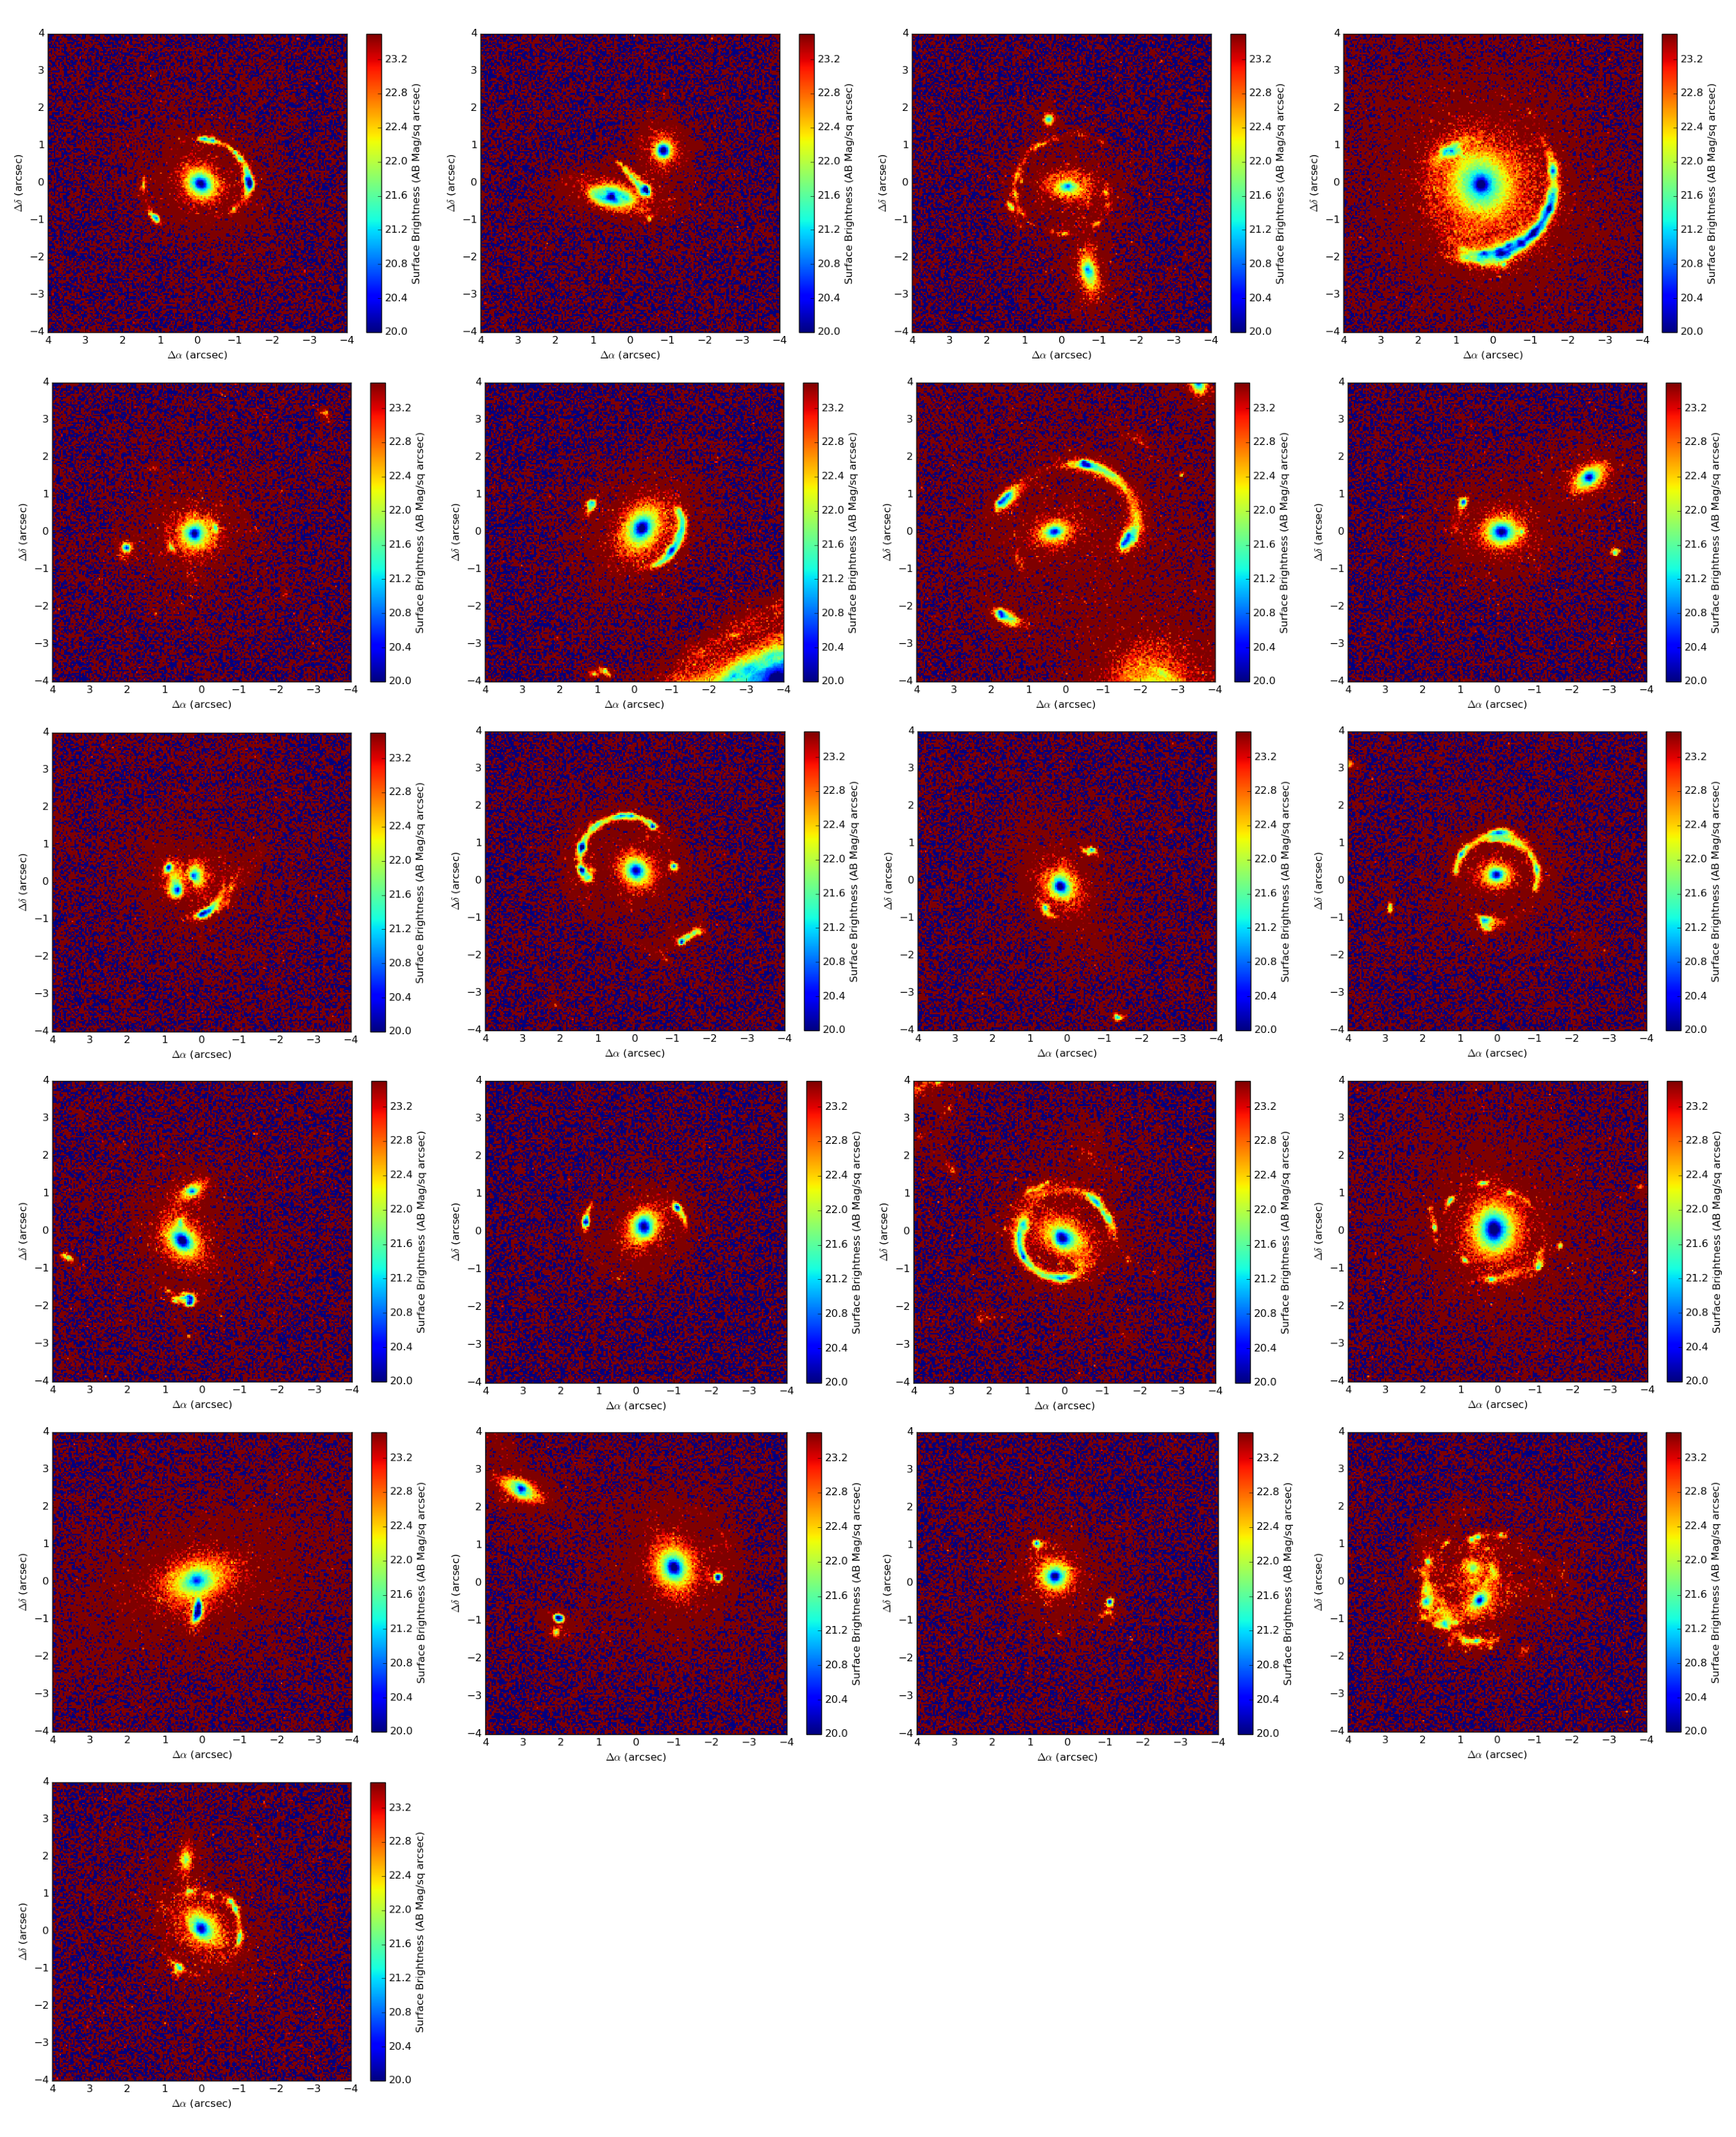
\includegraphics[width=\textwidth]{sample.pdf}
\caption{The WFC3 F606W imaging with the {\it HST} of each candidate gravitational lens. The cut-outs are $4\times4$ arcsec$^2$ is area, and the surface brightness scale is in AB magnitudes~arcsec$^{-2}$. {\bf Names and redshifts to be added.}}
\label{fig:sample}
\end{center}     
 \end{figure*}
=======
%\begin{figure*}
%\begin{center} 
%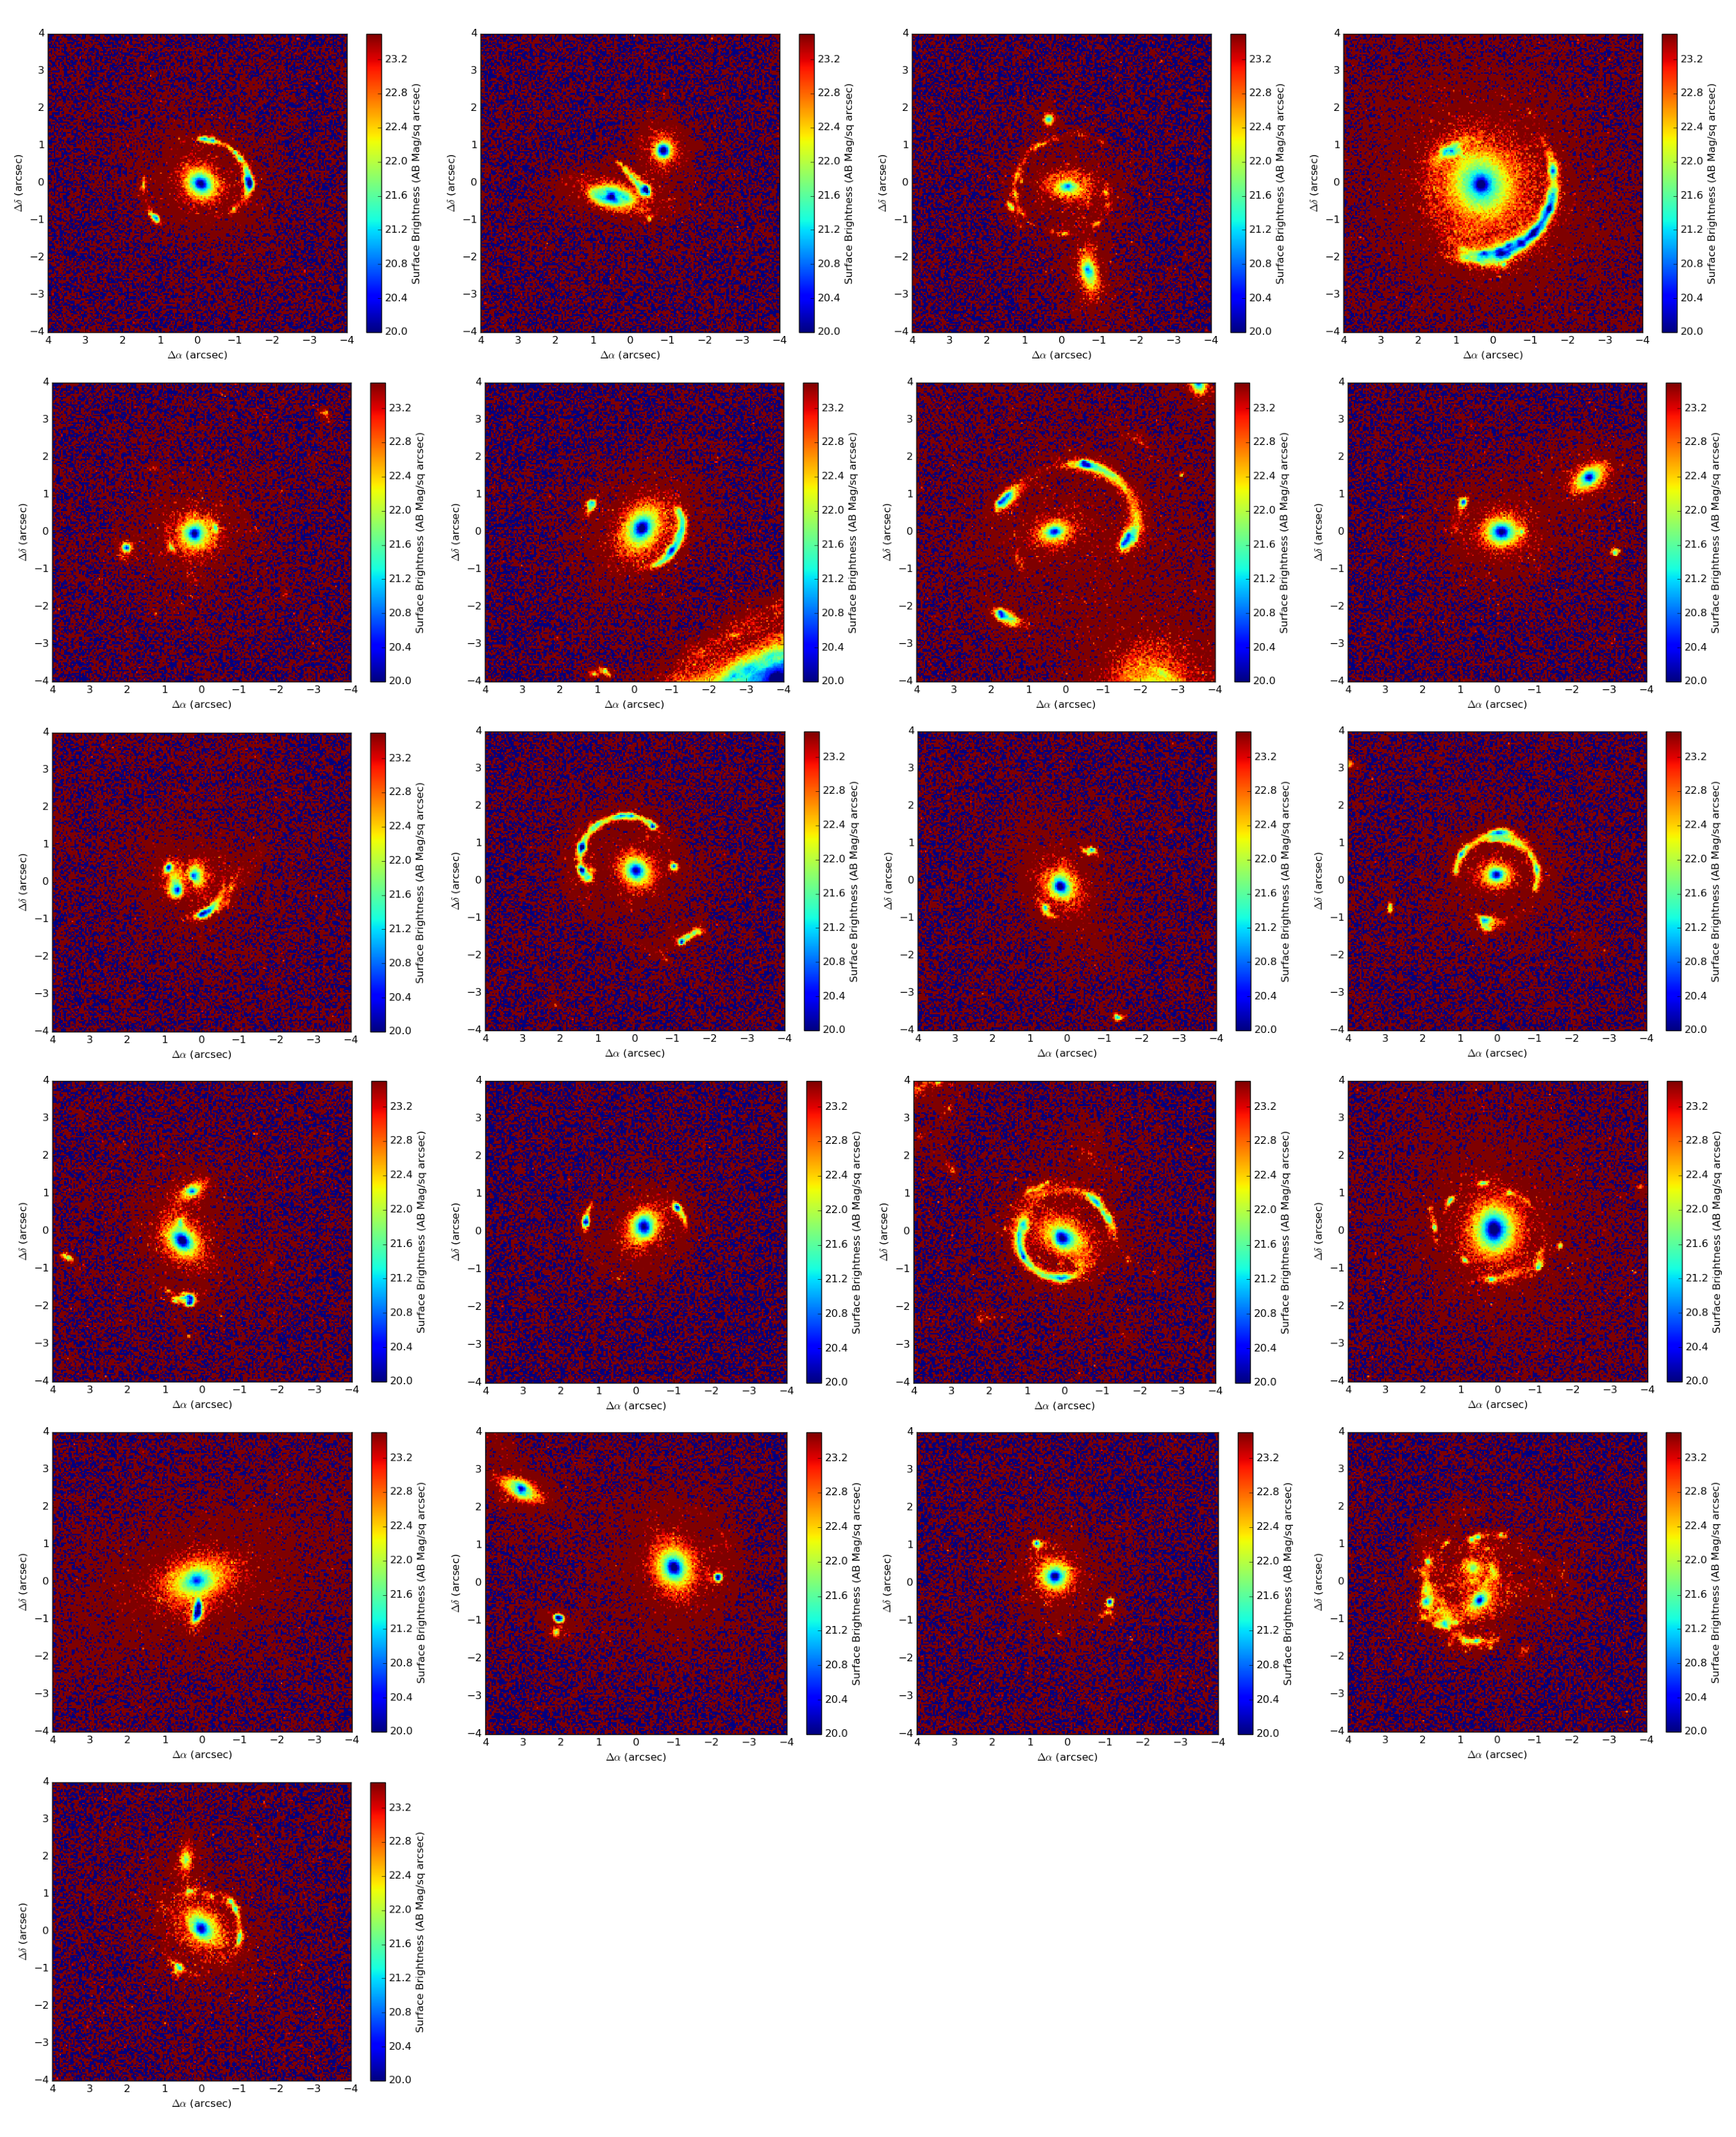
\includegraphics[width=\textwidth]{sample.pdf}
%\caption{The WFC3 F606W imaging with the {\it HST} of each candidate gravitational lens. The cut-outs are $4\times4$ arcsec$^2$ is area, and the surface brightness scale is in AB magnitudes~arcsec$^{-2}$. {\bf Names and redshifts to be added.}}
%\label{fig:sample}
%\end{center}     
% \end{figure*}
>>>>>>> origin/master

%Optical data as the considered sample, can allow us to detect substructures with mass in the range $10^7 - 10^8 M_{\odot}$ given their resolution; lower mass substructures can be detected using interferometric data that can take advantage of a higher resolution.
%The nature of the lensed galaxies is carefully selected to increase our sensitivity to the presence of substructures. Lyman-alpha emitters (LAEs) consist of inhomogeneous distribution of star forming knots and are often composed by distinct (components) units merging into one object. Given their structure, they present an extremely lumpy and discontinuous brightness profile which we can exploit to enhance the capability of identifying a substructure, as follows. Provided that the latter is located in the lens galaxy main halo and in correspondence of the Einstein ring, its presence would lead to a distortion in the brightness distribution of the lensed images. This local brightness perturbation will be more evident the more lumpy is the original unperturbed brightness profile in the same way changes in the positions of bricks in a wall are more easily identified if neighbouring bricks are differently coloured.

\section{Lens Modelling}

The gravitational lens modelling and source reconstruction of each system was performed using the Bayesian pixelated technique developed by \citet{V09}. Briefly, the mass density distribution of the lens is parametrized with an elliptical power-law profile (plus external shear) with a total of eight free parameters,
\begin{equation}\label{massdensity}
\kappa\left ( x,y \right ) = \frac{\kappa_0 \left ( 2 - \frac{\gamma}{2} \right ) q^{\gamma - 3/2}}{2 \left ( q^2 \left ( x^2 + r_c^2 \right ) + y^2\right )^{\left ( \gamma - 1 \right )/2}}\,, 
\end{equation}
where $\kappa$ is the dimensionless surface mass density (as a function of position $x,y$), $\kappa_0$ is the surface mass density normalization, $q$ is the axial ratio of the elliptical mass distribution, $\gamma$ is the radial slope of the mass density profile and $r_c$ is the core-radius. In addition, the position angle of the elliptical mass distribution ($\theta$), and the shear strength ($\Gamma$) and positional angle ($\Gamma_\theta$) as also solved for. The dimensionless surface mass density and the Einstein radius ($R_{\rm{ein}}$) are related to each other via,
\begin{equation}\label{einsteinradius}
R_{\rm{ein}} = \left ( \frac{\kappa_0 \left ( 2 - \frac{\gamma}{2} \right ) q^{\left ( \gamma - 2 \right )/2}}{3 - \gamma} \right )^{1/\left ( \gamma - 1 \right )}\,.
\end{equation}

The surface brightness distribution of the foreground gravitational lens is simultaneously modelled with the mass distribution and is parametrised using elliptical Sersic profiles 
\begin{equation}
I \left ( r \right ) = I_0 \exp \left [  \left (  - bn  \left (  \frac{r}{R_e} \right ) ^ {1/n} \right )  - 1.0   \right ]\,,
\end{equation}
where $I(r)$ is the surface brightness at radius $r$, $I_0$ is the surface brightness normalization, $R_{e}$ is the effective radius, $n$ is the Sersic index and $b$ is ??.
%\begin{equation}
%r = \sqrt{q_l^2  x_l ^2 + y_l ^2}\,.
%\end{equation}

The surface brightness distribution of the (lensing corrected) background source is instead reconstructed using a magnification-adaptive Delaunay tessellation and is characterised by a form and level of regularisation, $\mathbf{R_s}$ and $\lambda_s$ \citep[see][for a more detailed description]{V09,V14a}. This provides a pixellated surface brightness distribution for the reconstructed source that is free from any parameterised assumptions, such as Sersic or Gaussian light profiles, that may not fully account for the clumpy nature of the rest-frame ultraviolet emission from the BLAEs sources.

The modelling procedure is performed in two steps: first we masked out the emission from the lens galaxy and, given the lensed surface brightness distribution $\bmath d$, we optimize for the lens mass parameters $\bmath \eta = \{\kappa_0,\theta,q,x,y,\gamma,\Gamma,\Gamma_{\theta}\}$ and the source regularisation level by maximising the posterior probability density, 
\begin{equation}\label{equ:posterior}
    P(\lambda_{\rm{s}},\bmath \eta\,|\,\bmath d,\mathbf
      R_{\rm{s}})=\frac{P(\bmath d\,|\,\lambda_{\rm{s}},\bmath \eta,\mathbf
      R_{\rm{s}})P(\lambda_{\rm{s}},\bmath \eta)}{P(\bmath d\,|\,\mathbf
      R_{\rm{s}})}\,.
\end{equation}
At each step of this optimization, the corresponding most probable source $\bmath s$ is obtained by maximising the probability density distribution 
\begin{equation}
    P\left(\bmath s\,|\,\bmath d,\lambda_{\rm{s}}\bmath \eta,\mathbf R_{\rm{s}}\right)=\frac{P(\bmath d \,|\,\bmath s,\bmath \eta)\, P(\bmath s\,|\,\lambda_{\rm{s}},\mathbf R_{\rm{s}})}{P(\bmath     d \,|\,\lambda_{\rm{s}},\bmath \eta,\mathbf R_{\rm{s}})}\,.
   \label{eq:evidence} 
 \end{equation}
Then, using this as a starting point, we parametrise the surface brightness distribution of the lens galaxy as a sum of multiple elliptical Sersic profiles, and optimise for the corresponding parameters, $\bmath \eta_l =\{....\}$ together with the background source surface brightness distribution. In the third and last step, we optimise simultaneously for the mass and the light distribution of the deflector and the source regularisation level.

\begin{table*}
\caption{Add caption here.}
\begin{tabular}{cccc}
\hline
 Name (SDSS) &$\rm{z_{lens}}$&$\rm{z_{src}}$&$\rm{R_{ein}}$[arcsec]\\
 \hline
$\rm{J0029+2544}$&0.587&2.450\\
$\rm{J0113+0250}$&0.623&2.609\\
$\rm{J0201+3228}$&0.396&2.821\\
$\rm{J0237-0641}$&0.486&2.249\\
$\rm{J0742+3341}$&0.494&2.363\\
$\rm{J0755+3445}$&0.722&2.634\\
$\rm{J0856+2010}$&0.507&2.233\\
$\rm{J0918+4518}$&0.524&2.344\\
$\rm{J0918+5104}$&0.581&2.403\\
$\rm{J1110+2808}$&0.607&2.399\\
$\rm{J1110+3649}$&0.733&2.502\\
$\rm{J1141+2216}$&0.586&2.762\\
$\rm{J1201+4743}$&0.563&2.126\\
$\rm{J1226+5457}$&0.498&2.732\\
$\rm{J1529+4015}$&0.531&2.792\\
$\rm{J2228+1205}$&0.530&2.832\\
$\rm{J2342-0120}$&0.527&2.265\\
 \hline
\end{tabular}
\label{tbl:list} 
\end{table*}


\begin{table*}
\caption{Add caption here. This table should contain the best parameters for the sersic models}
\begin{tabular}{cccc}
\hline
 Name (SDSS) &$\rm{n_{Ser}}$\\
 \hline

 \hline
\end{tabular}
\label{tbl:sersic} 
\end{table*}

\section{Results}
%As can be seen in figure \ref{plots}, some of our models present quite a few residuals in correspondence of the lens galaxy. This is due to the attempt we are making to fit a pixelated emission with an analytical profile and in some cases the lens brightness profile is not well approximated by a Sersic profile. For these systems the lens brightness distribution is fitted with a B-spline profile and subtracted from the data. The obtained images are modelled again to prove that the bad fitting of the Sersic is not compromising the goodness of our lens model.
%
%Furthermore our prior on the source regularisation changes according to the specific system. In some cases a correlation between the pixels is needed in the regin outside the mask to achieve a better modelling: the regularisation matrix is therefore no longer diagonal.

\begin{figure*}
\begin{center} 
\includegraphics[width = 16 cm]{fig1a.ps}
\includegraphics[width = 16 cm]{fig1e.ps}
\includegraphics[width = 16 cm]{fig1g.ps}
\includegraphics[width = 16 cm]{fig1l.ps}
\caption{From top to bottom: best models for the lens gravitational systems ..... From left to right: input data, reconstructed model, normalised image residuals and reconstructed source.}
\label{fig:J0252_smooth}
\end{center}     
 \end{figure*}
 
 \begin{figure*}
\begin{center} 
\includegraphics[width = 16 cm]{fig1m.ps}
\includegraphics[width = 16 cm]{fig1o.ps}
\includegraphics[width = 16 cm]{fig1r.ps}
\includegraphics[width = 16 cm]{fig1s.ps}
\caption{From top to bottom: best models for the lens gravitational systems ..... From left to right: input data, reconstructed model, normalised image residuals and reconstructed source.}
\label{fig:J0252_smooth}
\end{center}     
 \end{figure*}



\section{Discussion}
%A recent update has been implemented: the emission coming from the Sersic fitting in each pixel of the lens plane is included in the matrix with the lens potential components and therefore we otimise for both the mass and brightness distribution of the lens galaxy simultaneously.

%Each system is analysed in two steps: we first find the best smooth lens model fitting the lens galaxy emission with two or more sersic components. Once the best lens smooth model is found, comprehensive of the lens images and the lens galaxy, we keep it fixed and proceed to locally correct the lens potential to to identify the presence of any substructures, which we detected as local brightness perturbations of the initial model.
%
%The section is structure as follows: for each lens system we present the plots of the smooth models and the correspondent optimised parameters in a recap table. In case any substructure has been detected, we summarise the smooth model in a recap table and only show the plot for the relative detection.

% This section should spread over both columns
%\onecolumn
%\section{SDSSJ0029+2544}
%At a first attempt we obtained a bad fit for the distribution of the light of the lens galaxy in the region of the lens plane we selected with the mask. This is where the lensed images lie and initially the only region of the sky where we imposed the regularisation on the reconstructed source. On the other hand this selection led to noise fitting which was subsequently solved implementing a simultaneous fitting of the mass and the light of the lens galaxy and an active regularisation over all the region of the sky.
%%\begin{figure}
%%	\includegraphics[width=\columnwidth]{/Users/admin/Dropbox/Smooth_models/	filename}
%%    \caption{Smooth model for SDSSJ0029+2544 with plotted critical curves.}
% %   \label{fig:smooth0029+2544}
%%\end{figure}
%
%\begin{table}
%\resizebox{\textwidth}{!}{\begin{minipage}{\textwidth}
%	\centering
%	\caption{Optimised lens parameters for SDSSJ0029+2544.}
%	\label{tab:lens0024+2544}
%	\begin{tabular}{lcccccccr} % four columns, alignment for each
%	
%		\hline
%		
%		b & $\theta$ & f & x & y & qh & $\Gamma_{sh}$ & $\theta_{sh}$ & z \\
%		(arcsec) & ($\circ$) &  & (arcsec) & (arcsec) &  & $\Gamma_{sh}$ & ($\circ$) & \\
%		
%		\hline
%		
%		 &  &  &  &  &  &  &  &  \\
%		 
%		\hline
%		
%	\end{tabular}
%\end{minipage} }
%\end{table}
%
%\begin{table}
%\resizebox{\textwidth}{!}{\begin{minipage}{\textwidth}
%	\centering
%	\caption{Optimised sersic parameters for SDSSJ0029+2544.}
%	\label{tab:sersic0024+2544}
%	\begin{tabular}{lccccccr} % four columns, alignment for each
%	
%		\hline
%		
%		Component & $I_{tot}$ & $R_e$ & n & x & y & $\theta$ & f\\
%		  & $I_{tot}$ & (arcsec) &  & (arcsec) & (arcsec) & ($\circ$) & \\
%		  
%		\hline
%		
%		first &  &  &  &   &  &  & \\
%		second & &  &  &  &  &  & \\
%		
%		\hline
%		
%	\end{tabular}
%\end{minipage} }
%\end{table}
%
%
%% This section should spread over both columns
%\section{0113+0250}
%This system presents two lenses, one of which is visible in the top side of the image. The smooth model parameters were accordingly optimised and both the lens galaxies were fitted trough Sersic components. An additional emission is visible in the bottom left part the plot for which both the mass and the light were optimised for.
%
%%\begin{figure}
%%	\includegraphics[width=\columnwidth]{/Users/admin/Dropbox/Smooth_models/filename}
%%    \caption{Smooth model for SDSSJ0113+0250 with plotted critical curves.}
% %   \label{fig:smooth0113+0250}
%%\end{figure}
%
%\begin{table}
%\resizebox{\textwidth}{!}{\begin{minipage}{\textwidth}
%	\centering
%	\caption{Optimised lens parameters for SDSSJ0113+0250. The strength and the position angle of the shear were optimised once for both the lenses.}
%	\label{tab:lens0113+0250}
%	\begin{tabular}{lccccccccr} % four columns, alignment for each
%	
%		\hline
%		
%		 & b & $\theta$ & f & x & y & qh & $\Gamma_{sh}$ & $\theta_{sh}$ & z\\
%		 & (arcsec) & ($\circ$) &  & (arcsec) & (arcsec) &  & $\Gamma_{sh}$ & ($\circ$) & \\
%		 
%		\hline
%		
%		first lens &  &  &  &  &  &  &  &  & \\
%		second lens &  & 8 &  &  &  &  &  &  & \\
%		
%		\hline
%		
%	\end{tabular}
%\end{minipage} }
%\end{table}
%
%\begin{table}
%\resizebox{\textwidth}{!}{\begin{minipage}{\textwidth}
%	\centering
%	\caption{Optimised sersic parameters for 0113+0250.}
%	\label{tab:sersic0113+0250}
%	\begin{tabular}{lcccccccr} % four columns, alignment for each
%	
%		\hline
%		
%		Lens & Component & $I_{tot}$ & $R_e$ & n & x & y & $\theta$ & f\\
%		  & & $I_{tot}$ & (arcsec) &  & (arcsec) & (arcsec) & ($\circ$) & \\
%		  
%		\hline
%		
%		First & I &  &  &  &  &  &  & \\
%		& II &  &  &  &  &  &  & \\
%		& III &  &  &  &  &  &  & \\
%		& IV &  &  &  &  &  &  & \\
%		
%		\hline
%		
%		Second & I &   &  &  &  &  &  & \\
%		& II &  &  &   &  &  &  & \\
%		
%		\hline
%		
%	\end{tabular}
%\end{minipage} }
%\end{table}
%
%
%
%
%\section{SDSSJ0237-0641}
%
%%\begin{figure}
%%	\includegraphics[width=\columnwidth]{/Users/admin/Dropbox/Smooth_models/	filename}
%%    \caption{Smooth model for SDSSJ0237-0641 with plotted critical curves.}
% %   \label{fig:smooth0237-0641}
%%\end{figure}
%
%\begin{table}
%\resizebox{\textwidth}{!}{\begin{minipage}{\textwidth}
%	\centering
%	\caption{Optimised lens parameters for SDSSJ0237-0641.}
%	\label{tab:lens0237-0641}
%	\begin{tabular}{lcccccccr} % four columns, alignment for each
%	
%		\hline
%		
%		b & $\theta$ & f & x & y & qh & $\Gamma_{sh}$ & $\theta_{sh}$ & z \\
%		(arcsec) & ($\circ$) &  & (arcsec) & (arcsec) &  & $\Gamma_{sh}$ & ($\circ$) & \\
%		
%		\hline
%		
%		 &  &  &  &  &  &  &  &  \\
%		 
%		\hline
%		
%	\end{tabular}
%\end{minipage} }
%\end{table}
%
%
%\begin{table}
%\resizebox{\textwidth}{!}{\begin{minipage}{\textwidth}
%	\centering
%	\caption{Optimised sersic parameters for SDSSJ0237-0641.}
%	\label{tab:sersic0237-0641}
%	\begin{tabular}{lccccccr} % four columns, alignment for each
%	
%		\hline
%		
%		Component & $I_{tot}$ & $R_e$ & n & x & y & $\theta$ & f\\
%		  & $I_{tot}$ & (arcsec) &  & (arcsec) & (arcsec) & ($\circ$) & \\
%		  
%		\hline
%		
%		first &  &  &  &   &  &  & \\
%		second & &  &  &  &  &  & \\
%		
%		\hline
%		
%	\end{tabular}
%\end{minipage} }
%\end{table}
%
%
%
%\section{SDSSJ0742+3341}
%
%%\begin{figure}
%%	\includegraphics[width=\columnwidth]{/Users/admin/Dropbox/Smooth_models/	filename}
%%    \caption{Smooth model for SDSSJ0742+3341 with plotted critical curves.}
% %   \label{fig:smooth0742+3341}
%%\end{figure}
%
%\begin{table}
%\resizebox{\textwidth}{!}{\begin{minipage}{\textwidth}
%	\centering
%	\caption{Optimised lens parameters for SDSSJ0742+3341.}
%	\label{tab:lens0742+3341}
%	\begin{tabular}{lcccccccr} % four columns, alignment for each
%	
%		\hline
%		
%		b & $\theta$ & f & x & y & qh & $\Gamma_{sh}$ & $\theta_{sh}$ & z \\
%		(arcsec) & ($\circ$) &  & (arcsec) & (arcsec) &  & $\Gamma_{sh}$ & ($\circ$) & \\
%		
%		\hline
%		
%		 &  &  &  &  &  &  &  &  \\
%		 
%		\hline
%		
%	\end{tabular}
%\end{minipage} }
%\end{table}
%
%
%\begin{table}
%\resizebox{\textwidth}{!}{\begin{minipage}{\textwidth}
%	\centering
%	\caption{Optimised sersic parameters for SDSSJ0742+3341.}
%	\label{tab:sersic0742+3341}
%	\begin{tabular}{lccccccr} % four columns, alignment for each
%	
%		\hline
%		
%		Component & $I_{tot}$ & $R_e$ & n & x & y & $\theta$ & f\\
%		  & $I_{tot}$ & (arcsec) &  & (arcsec) & (arcsec) & ($\circ$) & \\
%		  
%		\hline
%		
%		first &  &  &  &   &  &  & \\
%		second & &  &  &  &  &  & \\
%		
%		\hline
%		
%	\end{tabular}
%\end{minipage} }
%\end{table}
%
%\section{SDSSJ0918+4518}
%
%%\begin{figure}
%%	\includegraphics[width=\columnwidth]{/Users/admin/Dropbox/Smooth_models/	filename}
%%    \caption{Smooth model for SDSSJ0918+4518 with plotted critical curves.}
% %   \label{fig:smooth0918+4518}
%%\end{figure}
%
%\begin{table}
%\resizebox{\textwidth}{!}{\begin{minipage}{\textwidth}
%	\centering
%	\caption{Optimised lens parameters for SDSSJ0918+4518.}
%	\label{tab:lens0918+4518}
%	\begin{tabular}{lcccccccr} % four columns, alignment for each
%	
%		\hline
%		
%		b & $\theta$ & f & x & y & qh & $\Gamma_{sh}$ & $\theta_{sh}$ & z \\
%		(arcsec) & ($\circ$) &  & (arcsec) & (arcsec) &  & $\Gamma_{sh}$ & ($\circ$) & \\
%		
%		\hline
%		
%		 &  &  &  &  &  &  &  &  \\
%		 
%		\hline
%		
%	\end{tabular}
%\end{minipage} }
%\end{table}
%
%\begin{table}
%\resizebox{\textwidth}{!}{\begin{minipage}{\textwidth}
%	\centering
%	\caption{Optimised sersic parameters for both the lenses of SDSSJ0918+4518. The strength and the position angle of the shear were optimised once for both the lenses.}
%	\label{tab:sersic0918+4518}
%	\begin{tabular}{lcccccccr} % four columns, alignment for each
%	
%		\hline
%		
%		Lens & Component & $I_{tot}$ & $R_e$ & n & x & y & $\theta$ & f\\
%		  & & $I_{tot}$ & (arcsec) &  & (arcsec) & (arcsec) & ($\circ$) & \\
%		  
%		\hline
%		
%		First & I &  &  &  &  &  &  & \\
%		& II &  &  &  &  &  &  & \\
%		& III &  &  &  &  &  &  & \\
%		& IV &  &  &  &  &  &  & \\
%		
%		\hline
%		
%		Second & I &   &  &  &  &  &  & \\
%		& II &  &  &   &  &  &  & \\
%		
%		\hline
%		
%	\end{tabular}
%\end{minipage} }
%\end{table}
%
%
%
%\section{SDSSJ0918+5104}
%The configuration of this system is peculiar. The high value for the shear in table \ref{tab:lens0918+5104} is responsible for the stripping from the original configuration of the counterimage in the bottom right of the plot.
% 
% %\begin{figure}
%%	\includegraphics[width=\columnwidth]{/Users/admin/Dropbox/Smooth_models/	filename}
%%    \caption{Smooth model for SDSSJ0918+5104 with plotted critical curves.}
% %   \label{fig:smooth0918+5104}
%%\end{figure}
% 
%\begin{table}
%\resizebox{\textwidth}{!}{\begin{minipage}{\textwidth}
%	\centering
%	\caption{Optimised lens parameters for SDSSJ0918+5104.}
%	\label{tab:lens0918+5104}
%	\begin{tabular}{lcccccccr} % four columns, alignment for each
%	
%		\hline
%		
%		b & $\theta$ & f & x & y & qh & $\Gamma_{sh}$ & $\theta_{sh}$ & z \\
%		(arcsec) & ($\circ$) &  & (arcsec) & (arcsec) &  & $\Gamma_{sh}$ & ($\circ$) & \\
%		
%		\hline
%		
%		 &  &  &  &  &  &  &  &  \\
%		 
%		\hline
%		
%	\end{tabular}
%\end{minipage} }
%\end{table}
%
%\begin{table}
%\resizebox{\textwidth}{!}{\begin{minipage}{\textwidth}
%	\centering
%	\caption{Optimised sersic parameters for SDSSJ0918+5104.}
%	\label{tab:sersic0918+5104}
%	\begin{tabular}{lccccccr} % four columns, alignment for each
%	
%		\hline
%		
%		Component & $I_{tot}$ & $R_e$ & n & x & y & $\theta$ & f\\
%		  & $I_{tot}$ & (arcsec) &  & (arcsec) & (arcsec) & ($\circ$) & \\
%		  
%		\hline
%		
%		first &  &  &  &   &  &  & \\
%		second & &  &  &  &  &  & \\
%		
%		\hline
%		
%	\end{tabular}
%\end{minipage} }
%\end{table}
%
%
%\section{SDSSJ1201+4743}
%
% %\begin{figure}
%%	\includegraphics[width=\columnwidth]{/Users/admin/Dropbox/Smooth_models/	filename}
%%    \caption{Smooth model for SDSSJ1201+4743 with plotted critical curves.}
% %   \label{fig:smooth1201+4743}
%%\end{figure}
%
%\begin{table}
%\resizebox{\textwidth}{!}{\begin{minipage}{\textwidth}
%	\centering
%	\caption{Optimised lens parameters for SDSSJ1201+4743.}
%	\label{tab:lens1201+4743}
%	\begin{tabular}{lcccccccr} % four columns, alignment for each
%	
%		\hline
%		
%		b & $\theta$ & f & x & y & qh & $\Gamma_{sh}$ & $\theta_{sh}$ & z \\
%		(arcsec) & ($\circ$) &  & (arcsec) & (arcsec) &  & $\Gamma_{sh}$ & ($\circ$) & \\
%		
%		\hline
%		
%		 &  &  &  &  &  &  &  &  \\
%		 
%		\hline
%		
%	\end{tabular}
%\end{minipage} }
%\end{table}
%
%\begin{table}
%\resizebox{\textwidth}{!}{\begin{minipage}{\textwidth}
%	\centering
%	\caption{Optimised sersic parameters for SDSSJ1201+4743.}
%	\label{tab:sersic1201+4743}
%	\begin{tabular}{lccccccr} % four columns, alignment for each
%	
%		\hline
%		
%		Component & $I_{tot}$ & $R_e$ & n & x & y & $\theta$ & f\\
%		  & $I_{tot}$ & (arcsec) &  & (arcsec) & (arcsec) & ($\circ$) & \\
%		  
%		\hline
%		
%		first &  &  &  &   &  &  & \\
%		second & &  &  &  &  &  & \\
%		
%		\hline
%		
%	\end{tabular}
%\end{minipage} }
%\end{table}
%
%\section{SDSSJ2342-0120}
%
% %\begin{figure}
%%	\includegraphics[width=\columnwidth]{/Users/admin/Dropbox/Smooth_models/	filename}
%%    \caption{Smooth model for SDSSJ2342-0120 with plotted critical curves.}
% %   \label{fig:smooth2342-0120}
%%\end{figure}
%
%\begin{table}
%\resizebox{\textwidth}{!}{\begin{minipage}{\textwidth}
%	\centering
%	\caption{Optimised lens parameters for SDSSJ2342-0120.}
%	\label{tab:lens2342-0120}
%	\begin{tabular}{lcccccccr} % four columns, alignment for each
%	
%		\hline
%		
%		b & $\theta$ & f & x & y & qh & $\Gamma_{sh}$ & $\theta_{sh}$ & z \\
%		(arcsec) & ($\circ$) &  & (arcsec) & (arcsec) &  & $\Gamma_{sh}$ & ($\circ$) & \\
%		
%		\hline
%		
%		 &  &  &  &  &  &  &  &  \\
%		 
%		\hline
%		
%	\end{tabular}
%\end{minipage} }
%\end{table}
%
%\begin{table}
%\resizebox{\textwidth}{!}{\begin{minipage}{\textwidth}
%	\centering
%	\caption{Optimised sersic parameters for SDSSJ2342-0120.}
%	\label{tab:sersic2342-0120}
%	\begin{tabular}{lccccccr} % four columns, alignment for each
%	
%		\hline
%		
%		Component & $I_{tot}$ & $R_e$ & n & x & y & $\theta$ & f\\
%		  & $I_{tot}$ & (arcsec) &  & (arcsec) & (arcsec) & ($\circ$) & \\
%		  
%		\hline
%		
%		first &  &  &  &   &  &  & \\
%		second & &  &  &  &  &  & \\
%		
%		\hline
%		
%	\end{tabular}
%\end{minipage} }
%\end{table}
%
%\section{SDSSJ1110+2808}
%
% %\begin{figure}
%%	\includegraphics[width=\columnwidth]{/Users/admin/Dropbox/Smooth_models/	filename}
%%    \caption{Smooth model for SDSSJ1110+2808 with plotted critical curves.}
% %   \label{fig:smooth1110+2808}
%%\end{figure}
%
%\begin{table}
%\resizebox{\textwidth}{!}{\begin{minipage}{\textwidth}
%	\centering
%	\caption{Optimised lens parameters for SDSSJ1110+2808.}
%	\label{tab:lens1110+2808}
%	\begin{tabular}{lcccccccr} % four columns, alignment for each
%	
%		\hline
%		
%		b & $\theta$ & f & x & y & qh & $\Gamma_{sh}$ & $\theta_{sh}$ & z \\
%		(arcsec) & ($\circ$) &  & (arcsec) & (arcsec) &  & $\Gamma_{sh}$ & ($\circ$) & \\
%		
%		\hline
%		
%		 &  &  &  &  &  &  &  &  \\
%		 
%		\hline
%		
%	\end{tabular}
%\end{minipage} }
%\end{table}
%
%\begin{table}
%\resizebox{\textwidth}{!}{\begin{minipage}{\textwidth}
%	\centering
%	\caption{Optimised sersic parameters for SDSSJ1110+2808.}
%	\label{tab:sersic1110+2808}
%	\begin{tabular}{lccccccr} % four columns, alignment for each
%	
%		\hline
%		
%		Component & $I_{tot}$ & $R_e$ & n & x & y & $\theta$ & f\\
%		  & $I_{tot}$ & (arcsec) &  & (arcsec) & (arcsec) & ($\circ$) & \\
%		  
%		\hline
%		
%		first &  &  &  &   &  &  & \\
%		second & &  &  &  &  &  & \\
%		
%		\hline
%		
%	\end{tabular}
%\end{minipage} }
%\end{table}
%
%
%\section{SDSSJ1110+3649}
%
% %\begin{figure}
%%	\includegraphics[width=\columnwidth]{/Users/admin/Dropbox/Smooth_models/	filename}
%%    \caption{Smooth model for SDSSJ1110+3649 with plotted critical curves.}
% %   \label{fig:smooth1110+36498}
%%\end{figure}
%
%\begin{table}
%\resizebox{\textwidth}{!}{\begin{minipage}{\textwidth}
%	\centering
%	\caption{Optimised lens parameters for SDSSJ1110+3649.}
%	\label{tab:lens1110+3649}
%	\begin{tabular}{lcccccccr} % four columns, alignment for each
%	
%		\hline
%		
%		b & $\theta$ & f & x & y & qh & $\Gamma_{sh}$ & $\theta_{sh}$ & z \\
%		(arcsec) & ($\circ$) &  & (arcsec) & (arcsec) &  & $\Gamma_{sh}$ & ($\circ$) & \\
%		
%		\hline
%		
%		 &  &  &  &  &  &  &  &  \\
%		 
%		\hline
%		
%	\end{tabular}
%\end{minipage} }
%\end{table}
%
%\begin{table}
%\resizebox{\textwidth}{!}{\begin{minipage}{\textwidth}
%	\centering
%	\caption{Optimised sersic parameters for SDSSJ1110+3649.}
%	\label{tab:sersic1110+3649}
%	\begin{tabular}{lccccccr} % four columns, alignment for each
%	
%		\hline
%		
%		Component & $I_{tot}$ & $R_e$ & n & x & y & $\theta$ & f\\
%		  & $I_{tot}$ & (arcsec) &  & (arcsec) & (arcsec) & ($\circ$) & \\
%		  
%		\hline
%		
%		first &  &  &  &   &  &  & \\
%		second & &  &  &  &  &  & \\
%		
%		\hline
%		
%	\end{tabular}
%\end{minipage} }
%\end{table}

\bibliographystyle{mnras}
\bibliography{reference.bib}

\end{document}
